\section{Introduzione}

\textcolor{red}{PARLA DEL CITOMETRO IN GENERALE E DEL PERCHè USARE L'APPROCCIO ECM}

\textcolor{blue}{\lipsum[1]}

\section{Background}

\begin{figure*}[h!]
	\begin{subfigure}{0.5\linewidth}
			\centering
				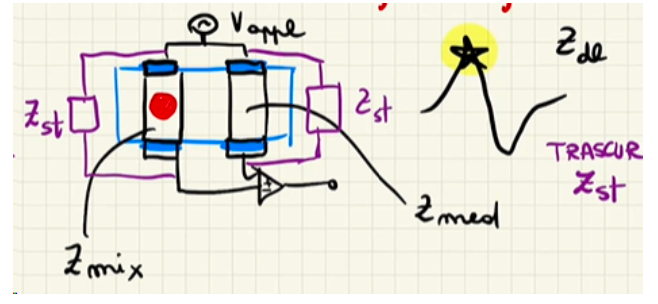
\includegraphics[width=0.95\linewidth]{figures/modello_circuitale}
				\caption{}
	\end{subfigure}\hfill
	\begin{subfigure}{0.5\linewidth}
	\centering
	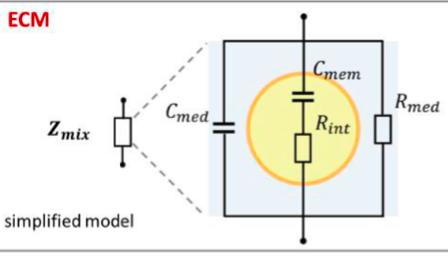
\includegraphics[width=0.5\linewidth]{figures/modello_circuitale1}
	\caption{}
\end{subfigure}\hfill
	\caption{Schema circuitale di misura nel citometro ad impedenza e tipico segnale (a); equivalente circuitale per cellula nel mezzo. Il segnale bipolare presenta il picco nel momento in cui la cellula passa tra le coppie parallele di elettrodi. Nello schema circuitale sono trascurate eventuali impedenze parassite.}
	\label{fig:modellocircuitale}
\end{figure*}



La modellazione tramite equivalente circuitale porta in contro la teoria delle miscele di Maxwell (MMT) per modellare le proprietà dielettriche cellulari.

Tale modello permette di descrivere il segnale ottenuto in un citometro ad impedenza ad elettrodi paralleli nel momento in cui la cellula si trova tra una coppia di elettrodi. La presenza della cellula tra gli elettrodi, insieme alla perturbazione del campo elettrico, genera un segnale di corrente differenziale che risulta proporzionale al diametro per il tramite del fattore di Clausis-Mossotti \cite{bibid}.

Nel seguente report verrà considerata una versione semplificata del segnale, pari a:

\begin{equation}
	S=r^{3} f_{C M}
\end{equation}

\subsection{Equivalenza circuitale}

Il circuito in \cref{fig:modellocircuitale} prevede l'applicazione di un potenziale agli elettrodi superiori e il campionamento del segnale dagli elettrodi inferiori, come corrente differenziale.

Osservando il percorso della corrente essa si troverà a passare per gli elettrodi e poi per il buffer conduttivo, eventualmente anche incontrando la cellula. Ognuno di questi materiali contribuirà con una sua impedenza.

Tali impedenze sono in serie e quindi il segnale misurato sarà:

\begin{equation}
	I_{\operatorname{d i f f}}=\frac{V_{\operatorname{a p p l}}}{Z_{\operatorname{m e d}}+2 Z_{d l}}-\frac{V_{\operatorname{a p p l}}}{Z_{\operatorname{m i x}}+2 Z_{d l}}
\end{equation}

Dove l'impedenza $Z_{\operatorname{m i x}}$ rappresenta l'insieme di cellula e buffer conduttivo e verrà descritta più avanti tramite MMT.

Inoltre, in questo segnale, riorganizzando i termini, compare una differenza di impedenza $\Delta Z=Z_{\operatorname{m i x}}-Z_{\operatorname{m e d}}$ pari proprio alla perturbazione indotta dalla cellula.  Tale termine inoltre risulta molto minore dell'impedenza del mezzo e questo ci permette di trascurare i termini quadratici e ottenere un segnale di corrente differenziale pari a:

\begin{equation}
\begin{aligned}
	I_{\operatorname{d i f f}}\approx &V_{\operatorname{a p p l}}\frac{Z_{\operatorname{m i x}} -Z_{\operatorname{m e d}}}{\left(Z_{\operatorname{m e d}} +2Z_{dl}\right)^2}\\
	=&  {V_{\operatorname{a p p l}}\over Z_{\operatorname{m e d}}^2} \frac{Z_{\operatorname{m i x}} -Z_{\operatorname{m e d}}}{\left(1+ 2{Z_{dl}\over Z_{\operatorname{m e d}} }\right)^2}
\end{aligned}
\end{equation}

L'impedenza di elettrodo è legata alla capacità superficiale $C_{dl}$ e alle dimensioni del volume del canale compreso tra le coppie. Risulta essere pari a:

\begin{equation}
	Z_{d l}=\frac{1}{j \omega C_{d l} w l}
\end{equation}

L'impedenza del mezzo viene espressa tramite la legge di Ohm, contestualizzandola in funzione del volume del canale:

\begin{equation}
	Z_{\operatorname{m e d}}=\frac{h}{\sigma^{*} l w k}={1\over \sigma^*}{1\over G}={1\over j\omega \varepsilon ^*}{1\over G}
\end{equation}

Portando in conto anche effetti di distorsione del campo elettrico tramite un coefficiente geometrico $G$. 

In generale, la permittività complessa è esprimibile come:

\begin{equation}
	\varepsilon^{*}=\varepsilon+\frac{\sigma}{j \omega}
\end{equation}

Tali considerazioni sono analoghe per l'impedenza del mix dove però la $\varepsilon^*_{\operatorname{m i x}}$ va stimata tramite la teoria delle miscele di Maxwell. 

\subsection{Maxwell's Mixtures theory}



\textcolor{blue}{\lipsum[1-4]}



\section{Risultati}

\textcolor{blue}{\lipsum[1-4]}





\section{Conclusioni}

\textcolor{blue}{\lipsum[1-2]}


\raggedbottom


\raggedbottom
\pagebreak
\section*{Disponiblità dei dati}

Il materiale è disponibile alla repository online del progetto: \url{https://github.com/mastroalex/ecm-mmt}.

\printbibliography[title=Riferimenti]
%\section*{References}

\clearpage
\onecolumn
\section*{Appendice}

